\hypertarget{group__xEventGroupSetBits}{}\section{x\+Event\+Group\+Set\+Bits}
\label{group__xEventGroupSetBits}\index{x\+Event\+Group\+Set\+Bits@{x\+Event\+Group\+Set\+Bits}}
Collaboration diagram for x\+Event\+Group\+Set\+Bits\+:\nopagebreak
\begin{figure}[H]
\begin{center}
\leavevmode
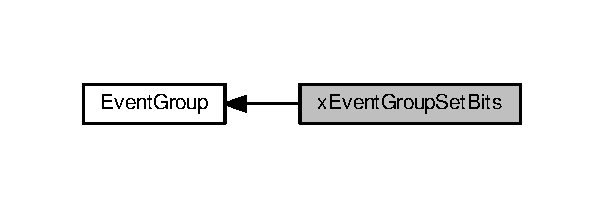
\includegraphics[width=290pt]{dd/d08/group__xEventGroupSetBits}
\end{center}
\end{figure}
\hyperlink{event__groups_8h}{event\+\_\+groups.\+h} 
\begin{DoxyPre}
   EventBits\_t \hyperlink{event__groups_8h_a02d7b3bb55f7e11d9c47116266c5fb2e}{xEventGroupSetBits( EventGroupHandle\_t xEventGroup, const EventBits\_t uxBitsToSet )};
\end{DoxyPre}


Set bits within an event group. This function cannot be called from an interrupt. \hyperlink{event__groups_8h_a62b68278abac6358369ae8e390988a02}{x\+Event\+Group\+Set\+Bits\+From\+I\+S\+R()} is a version that can be called from an interrupt.

Setting bits in an event group will automatically unblock tasks that are blocked waiting for the bits.


\begin{DoxyParams}{Parameters}
{\em x\+Event\+Group} & The event group in which the bits are to be set.\\
\hline
{\em ux\+Bits\+To\+Set} & A bitwise value that indicates the bit or bits to set. For example, to set bit 3 only, set ux\+Bits\+To\+Set to 0x08. To set bit 3 and bit 0 set ux\+Bits\+To\+Set to 0x09.\\
\hline
\end{DoxyParams}
\begin{DoxyReturn}{Returns}
The value of the event group at the time the call to \hyperlink{event__groups_8h_a02d7b3bb55f7e11d9c47116266c5fb2e}{x\+Event\+Group\+Set\+Bits()} returns. There are two reasons why the returned value might have the bits specified by the ux\+Bits\+To\+Set parameter cleared. First, if setting a bit results in a task that was waiting for the bit leaving the blocked state then it is possible the bit will be cleared automatically (see the x\+Clear\+Bit\+On\+Exit parameter of \hyperlink{event__groups_8h_aab9d5b405bc57b7624dcabe9a9a503db}{x\+Event\+Group\+Wait\+Bits()}). Second, any unblocked (or otherwise Ready state) task that has a priority above that of the task that called \hyperlink{event__groups_8h_a02d7b3bb55f7e11d9c47116266c5fb2e}{x\+Event\+Group\+Set\+Bits()} will execute and may change the event group value before the call to \hyperlink{event__groups_8h_a02d7b3bb55f7e11d9c47116266c5fb2e}{x\+Event\+Group\+Set\+Bits()} returns.
\end{DoxyReturn}
Example usage\+: 
\begin{DoxyPre}
  #define BIT\_0 ( 1 << 0 )
  #define BIT\_4 ( 1 << 4 )\end{DoxyPre}



\begin{DoxyPre}  void aFunction( EventGroupHandle\_t xEventGroup )
  \{
  EventBits\_t uxBits;\end{DoxyPre}



\begin{DoxyPre}    // Set bit 0 and bit 4 in xEventGroup.
    uxBits = xEventGroupSetBits(
                        xEventGroup,    // The event group being updated.
                        BIT\_0 | BIT\_4 );// The bits being set.\end{DoxyPre}



\begin{DoxyPre}    if( ( uxBits \& ( BIT\_0 | BIT\_4 ) ) == ( BIT\_0 | BIT\_4 ) )
    \{
        // Both bit 0 and bit 4 remained set when the function returned.
    \}
    else if( ( uxBits \& BIT\_0 ) != 0 )
    \{
        // Bit 0 remained set when the function returned, but bit 4 was
        // cleared.  It might be that bit 4 was cleared automatically as a
        // task that was waiting for bit 4 was removed from the Blocked
        // state.
    \}
    else if( ( uxBits \& BIT\_4 ) != 0 )
    \{
        // Bit 4 remained set when the function returned, but bit 0 was
        // cleared.  It might be that bit 0 was cleared automatically as a
        // task that was waiting for bit 0 was removed from the Blocked
        // state.
    \}
    else
    \{
        // Neither bit 0 nor bit 4 remained set.  It might be that a task
        // was waiting for both of the bits to be set, and the bits were
        // cleared as the task left the Blocked state.
    \}
  \}
  \end{DoxyPre}
 